\documentclass[a4paper,11pt]{article}

\usepackage[english]{babel}
\usepackage{mathrsfs, amssymb, amsmath, amsthm, enumerate}
\usepackage{verbatim,graphicx,geometry}
%\usetikzlibrary{arrows}
\usepackage[utf8]{inputenc}
\usepackage{authblk}
\usepackage[round]{natbib}
\bibliographystyle{plainnat}

\usepackage{hyperref}

\makeatletter
\def\@biblabel#1{\hspace*{-\labelsep}}
\makeatother
\geometry{left=1in,right=1
in,top=1in,bottom=1in}
\newdimen\dummy
\dummy=\oddsidemargin
\addtolength{\dummy}{72pt}
\marginparwidth=.5\dummy
\marginparsep=.1\dummy


\newcommand{\E}{\mathbb{E}}
\newcommand{\Var}{\mathrm{Var}}
\newcommand{\plim}{\overset{p}{\longrightarrow}}
\newcommand{\dlim}{\overset{d}{\longrightarrow}}

\begin{document}

\section*{Parameter Search}


\begin{table}[h!]
\centering
\begin{tabular}{llp{5cm}p{5cm}}
\hline \hline
Parameter & value & interpretation & Moment\\ \hline
$\gamma$ & 0.6 & Scale of GDP production & Labor share of GDP \\
$\epsilon$ & 2& Elasticity of intertemporal substitution & From misallocation paper   \\
$I$ & $e^{100}$ & initial number of inventors &  Match initial number of patents\\
$\nu$ & 2.8 & ratio of firms to inventors & average GDP growth \\
$g_1, g_2$&0.066, 0.02 & growth rates of population & patent number growth\\
$\eta^L$& 0 & reuse benefit & normalized \\
\hline \hline
\end{tabular}
\caption{Parameters matched before-hand.}
\end{table}

\begin{table}[h!]
\centering
\begin{tabular}{lll}
\hline \hline
Parameter & value & interpretation \\ \hline
$\eta^H$ & 0.3 & New technology benefit \\
$\eta^M$ & 0.07 & New combination benefit \\
$\tau$ & 500 & Shape parameter for idea distribution \\
$\xi$ & 200 & $1/\xi$ is the fraction of viable combinations \\
$\lambda $ & 1 & scale parameter of the cost distribution \\
$\kappa $ & 5  & shape parameter of the cost distribution \\
$\zeta$ & 0.012 & probability that tech line shuts down \\
\hline \hline
\end{tabular}
\caption{Parameters from patent type fraction moment matching}
\end{table}


\begin{table}[h!]
\centering
\begin{tabular}{|l|l|l|}
\hline
&\textbf{Data}&\textbf{Model}\\\hline
\textbf{new tech 1850}&0.4&0.41068\\\hline
\textbf{new comb 1850}&0.25&0.095672\\\hline
\textbf{reuse 1850}&0.35&0.49365\\\hline
\textbf{new tech 1900}&0.03&0.039405\\\hline
\textbf{new comb 1900}&0.45&0.41264\\\hline
\textbf{reuse 1900}&0.52&0.54795\\\hline
\textbf{new tech 1950}&0.02&0.030923\\\hline
\textbf{new comb 1950}&0.75&0.74522\\\hline
\textbf{reuse 1950}&0.33&0.22386\\\hline
\textbf{new tech 2000}&0.01&0.029089\\\hline
\textbf{new comb 2000}&0.8&0.81023\\\hline
\textbf{reuse 2000}&0.19&0.16069\\\hline
\textbf{reuse peak}&0.55&0.65526\\\hline
\end{tabular}

\caption{Moments (the missing column numbers are the moments I dropped relative to the old specification). Obs.: column 8 is not included as an argument in the objective function $\Rightarrow$ still under-identified.}
\end{table}


\begin{figure}[h!]
\begin{center}
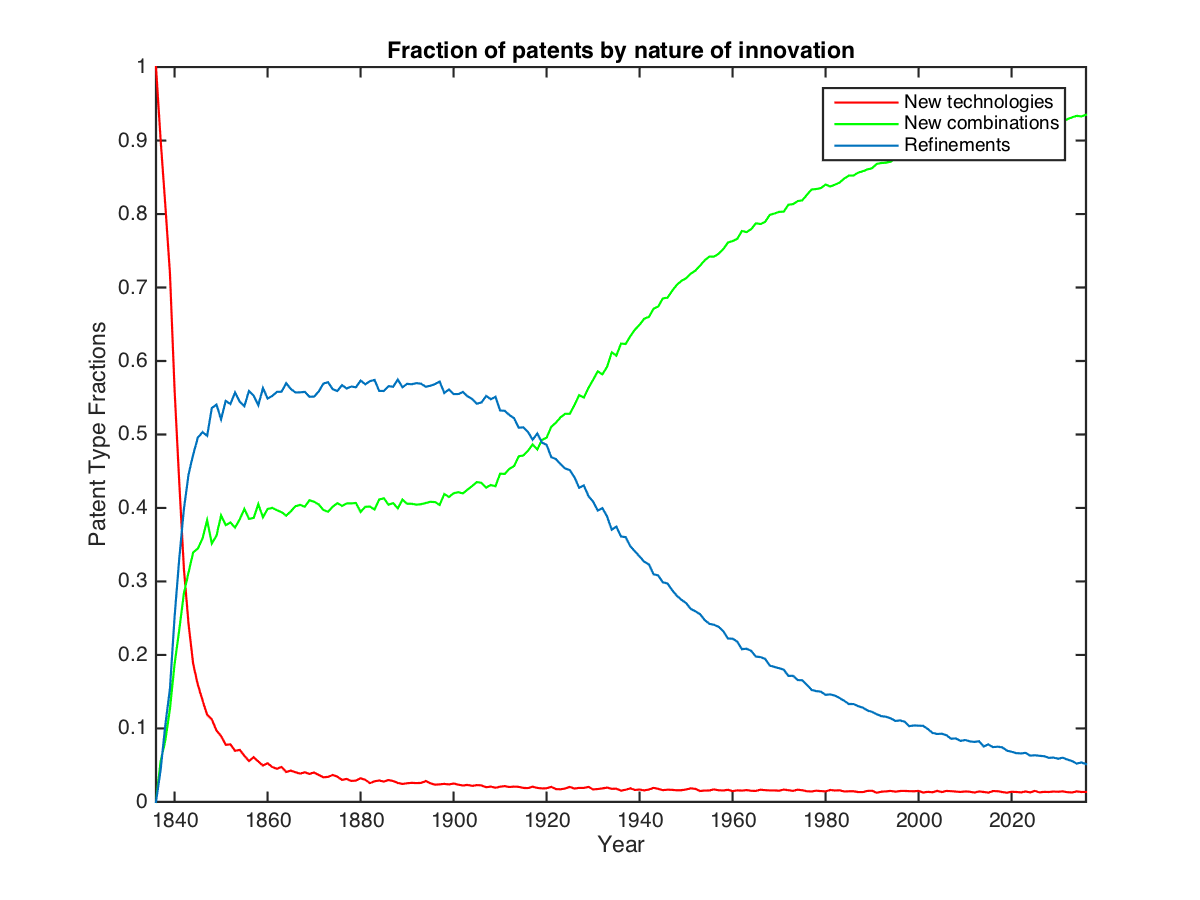
\includegraphics[scale=.8]{figures/patents.png}
\caption{Fraction of patents by type}
\end{center}
\end{figure}

\begin{figure}[h!]
\begin{center}
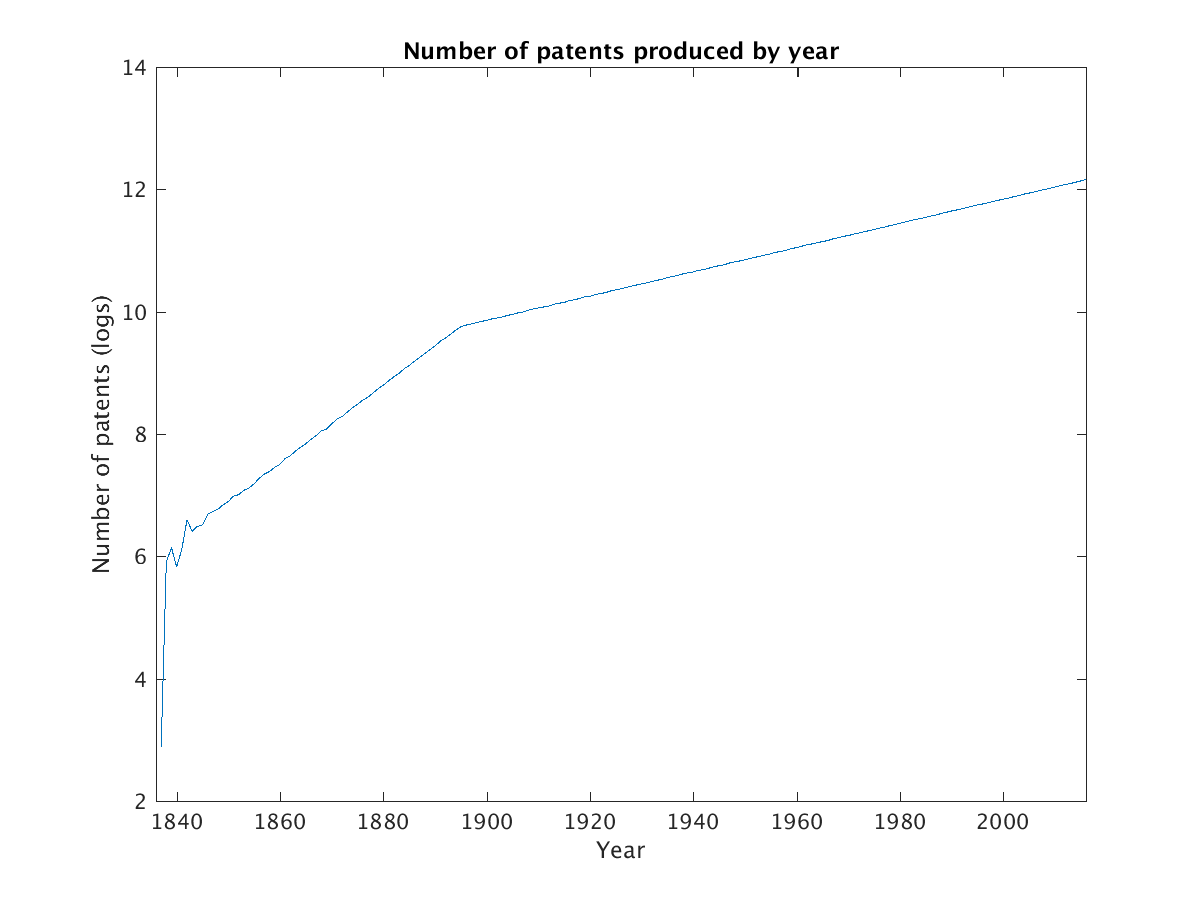
\includegraphics[scale=.8]{figures/num_pats.png}
\caption{Number of patents produced}
\end{center}
\end{figure}

\begin{figure}[h!]
\begin{center}
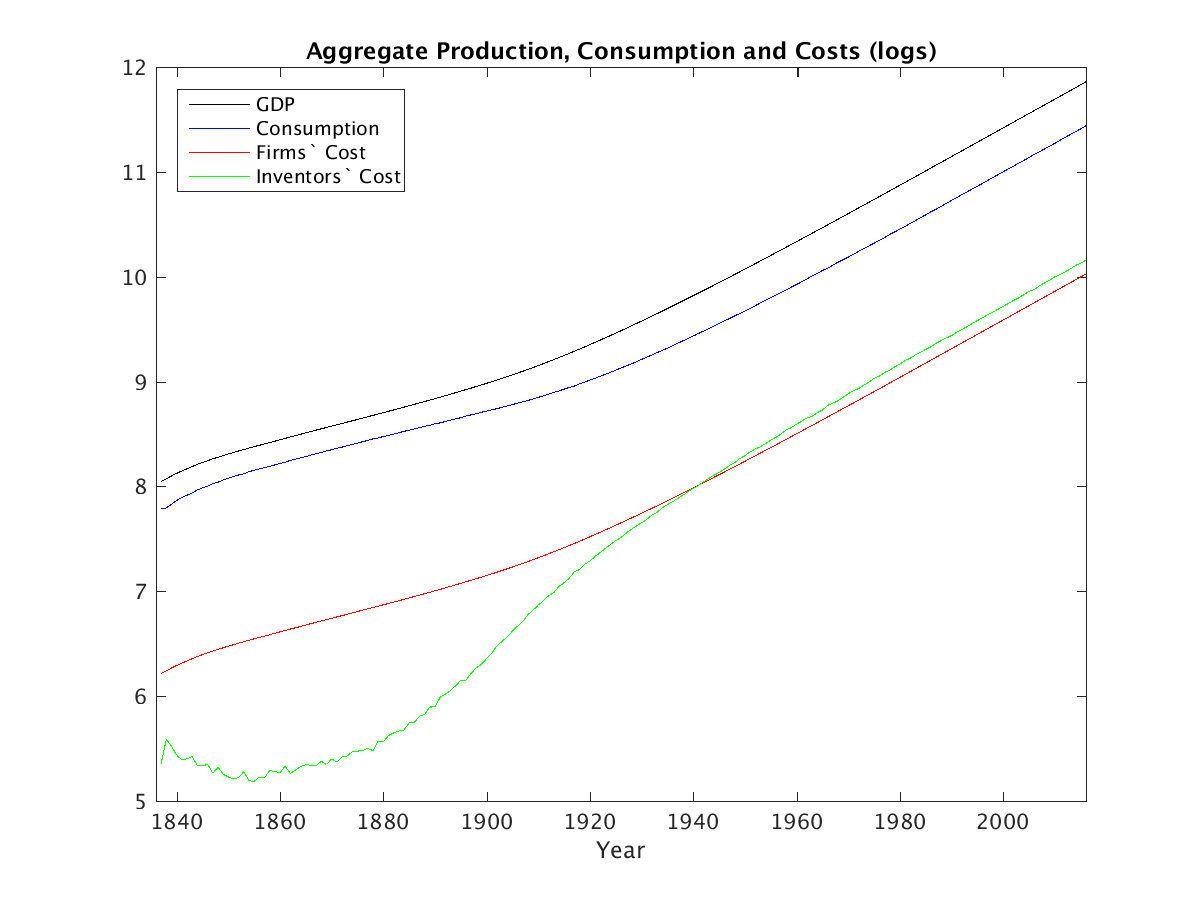
\includegraphics[scale=.8]{figures/aggregates.png}
\caption{Aggregate variables in the final goods market clearing}
\end{center}
\end{figure}

\begin{figure}[h!]
\begin{center}
\includegraphics[scale=.8]{figures/growth.png}
\caption{Rate of growth of the economy}
\end{center}
\end{figure}

\section{Welfare Counterfactuals}

\begin{figure}[h!]
\begin{center}
\includegraphics[scale=.8]{figures/Welfare_pp.png}
\caption{Difference in welfare gains between new combinations to new technology}
\end{center}
\end{figure}

\begin{figure}[h!]
\begin{center}
\includegraphics[scale=.8]{figures/Welfare_NT.png}
\caption{Welfare gains from subsidizing new technologies}
\end{center}
\end{figure}

\begin{figure}[h!]
\begin{center}
\includegraphics[scale=.8]{figures/Welfare_NC.png}
\caption{Welfare gains from subsidizing new combinations}
\end{center}
\end{figure}


\end{document}

\section*{Sensitivity analysis}

\begin{table}[h!]
\hspace*{-1cm}\begin{tabular}{lllllll}
\hline \hline
\textbf{Parameter changed}&\textbf{NC 1880}&\textbf{NT 1880}&\textbf{NC 1930}&\textbf{NT 1930}&\textbf{Peak of reuse} & \textbf{Year of peak}\\\hline
\textbf{$\eta^H$}&0.25314&0.077351&0.45259&0.040606&0.79891&1851\\\hline
\textbf{$\eta^M$}&0.44517&0.1036&0.63846&0.055556&0.62018&1850\\\hline
\textbf{$\tau$}&0.41794&0.093815&0.61242&0.05038&0.66305&1850\\\hline
\textbf{$\lambda$}&0.56153&0.11383&0.73459&0.061152&0.51344&1848\\\hline
\textbf{$\kappa$}&0.47448&0.10177&0.66667&0.054808&0.6135&1849\\\hline
\textbf{$\xi$}&0.48193&0.10102&0.66175&0.05405&0.59305&1849\\\hline
\textbf{Baseline}&0.4521&0.101&0.6416&0.0542&0.623&1849\\\hline
\textbf{data}&0.3&0.1&0.6&0.03&0.6&1870\\
\hline \hline
\end{tabular}
\caption{Variation in moments given 20\% decrease in parameter values.}
\end{table}

From table 3, $\eta^H$ and $\lambda$ are driving most of the change. $\tau$, $\kappa$ and $\xi$ also seem to have a considerable effect on the fraction of new combinations. $\eta^M$ has the weakest effect in all moments.

\section*{Rate of Growth}

\begin{figure}[h!]
\begin{center}
\includegraphics[scale=.8]{growth.png}
\caption{Growth rate of economy}
\end{center}
\end{figure}

Figure 2 has the rate of growth of the economy. It was computed by taking the average patent quality among firms. I chose the number of firms to yield an average growth rate of 2\%, which gave 683 firms. 

Until around 1845, the rate of growth seems to be affected the most by the movement of the fraction of new technologies. This feature can be somewhat ``artificial", happening mainly because we define the fraction of new technologies in 1836 to be equal to 1. Soon after that, this effect fades out and the rate of growth seems to stabilize around 2\%, the historical mean. Note that there is a slight increase in the rate of growth, as the fraction of new combinations increases as well. 

If we zoom in on the rate of growth starting at 1846 instead, we get figure 3:

\begin{figure}[h!]
\begin{center}
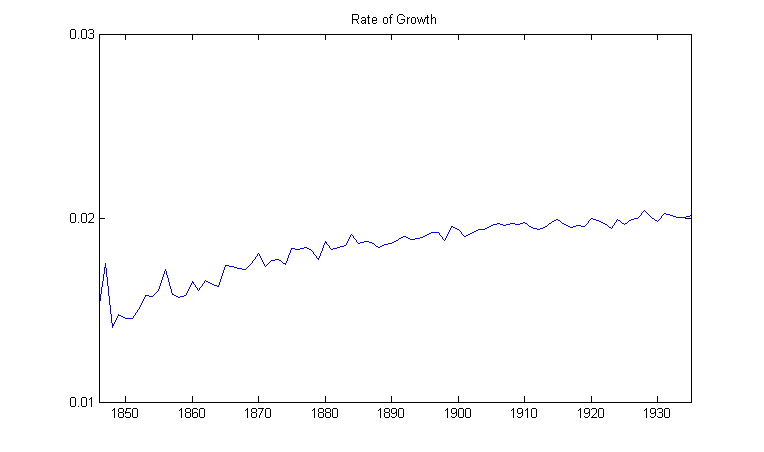
\includegraphics[scale=.8]{growth_zoom.png}
\caption{Growth rate of economy after 1846.}
\end{center}
\end{figure}



\end{document}